\documentclass[10pt,a4paper]{article}
\usepackage[utf8]{inputenc}
\usepackage{amsmath}
\usepackage{amsfonts}
\usepackage{amssymb}
\usepackage[margin=3cm]{geometry}
\usepackage{xspace}
\usepackage{enumerate}
\usepackage{graphicx}
\usepackage{hyperref}
\usepackage[sc]{mathpazo}
\linespread{1.05}         % Palladio needs more leading (space between lines)
\usepackage[T1]{fontenc}
\begin{document}

\def\ether{Ether\xspace}
\def\ie{{i.e.}\xspace}
\def\eg{{e.g.}\xspace}
\def\tld{{\sc tld}}
\def\tlds{\tld{s}\xspace}
\def\sld{{\sc sld}}
\def\slds{\sld{s}\xspace}
\def\icann{{\sc icann}\xspace}
\def\qrcode{{\sc qr}-code\xspace}
\def\qrcodes{\qrcode{s}\xspace}
\def\nfc{{\sc nfc}\xspace}
\def\dapp{{\sc da}pp\xspace}
\def\dapps{\dapp{s}\xspace}
\def\dao{{\sc dao}\xspace}
\def\daos{\dao{s}\xspace}
\def\ambedon{{\sc ambedon}\xspace}

\begin{center}
{\huge Assignment Management of 

Ethereum Domain Names}

\vspace{0.6cm}
{\small Aeron Buchanan, v1}
\end{center}

This document is to explore the need for, goals of and problems associated with the Ethereum domain name assignment.

Much appreciated input came from Gavin Wood, Vladislav Gluhovsky and Yanislav Malahov.

\section*{Overview}

An obvious use for a public consensus database, such as provided by Ethereum, is an alias lookup system. It was the first extension to the functionality of the bitcoin blockchain, realized in a fork called NameCoin. Gavin Wood added the "NameReg" contract to Ethereum testnets early on. For the Internet, there is, of course, the DNS system. The Bitalias protocol proposes an alias assignment system directly on the bitcoin lockchain. DNS, NameReg and BitAlias are for platform address aliases, whereas NameCoin is explicitly general purpose. 

An alias service on Ethereum will happen one way or another, so a sensible default should be provided. At least some economic analysis should inform the design. To this end, aliases on Ethereum, like DNS domain names, should not be treated as a scarce resource in general, but individually, by definition, they are uniquely scarce. As such, there is a hidden resource allocation problem to be solved in the running of such a service. Ethereum wants aliases to be used in a way that maximizes utility to the ecosystem (not, for example, to directly maximize any particular entity's profit), but there is no way to usefully judge or practically assess the use of an alias, hence using the word `hidden'. 

\begin{center}
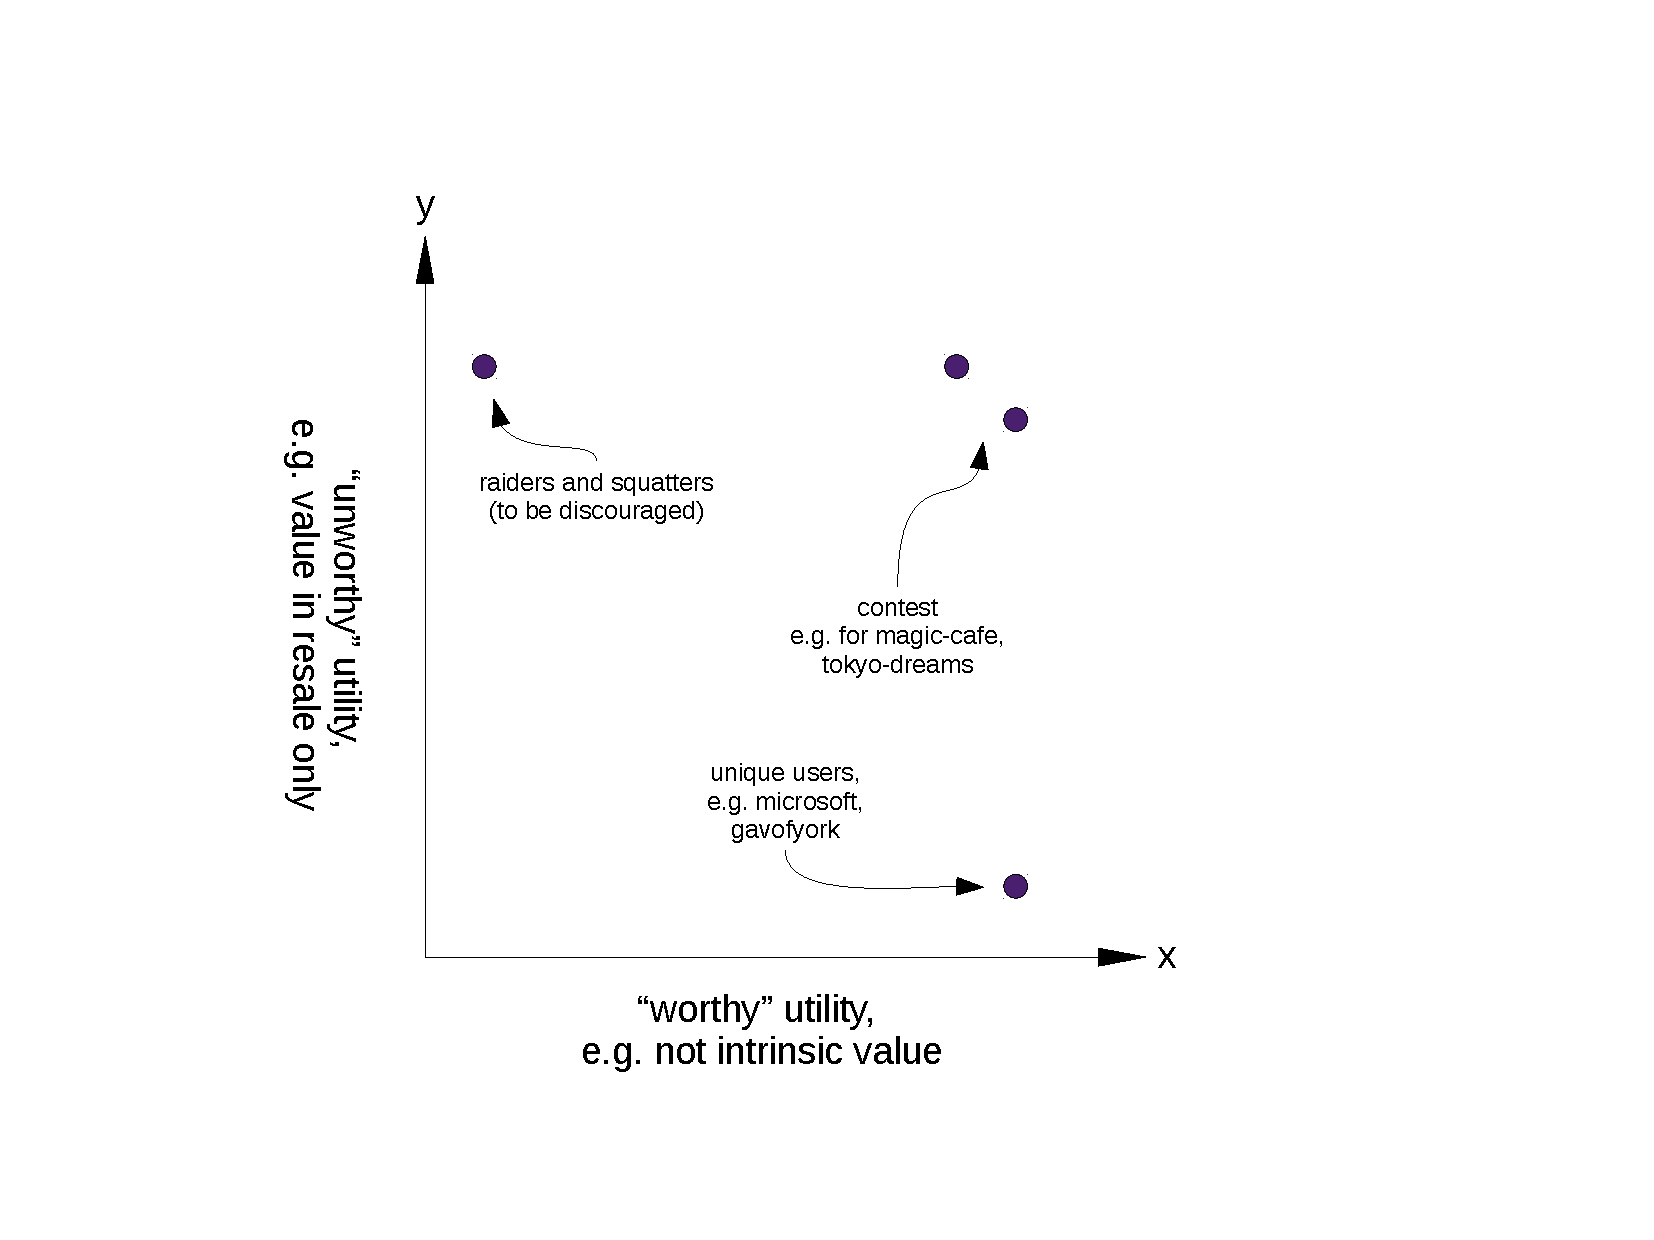
\includegraphics[trim=4.5cm 2.5cm 5.5cm 3cm, clip, width=7cm]{Diagrams/AliasUtility2D.pdf}
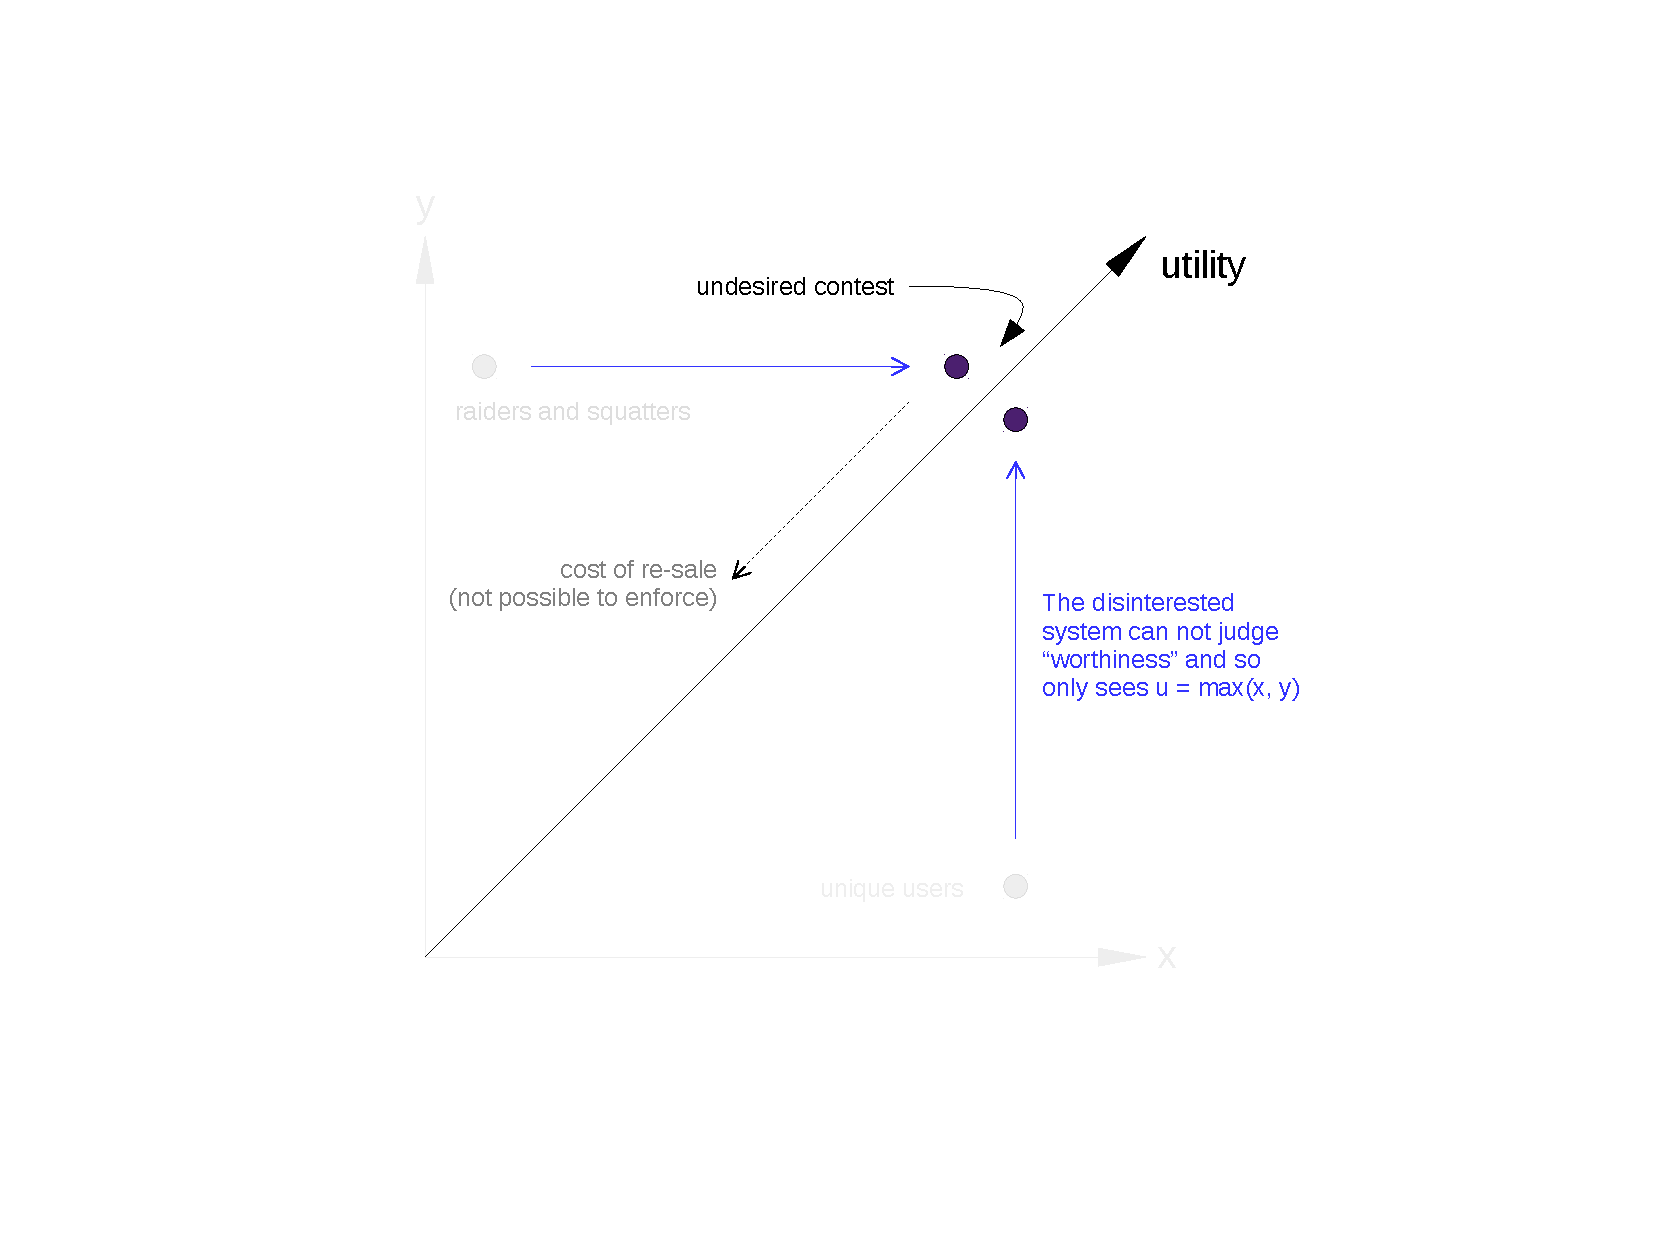
\includegraphics[trim=4.5cm 2.5cm 5.5cm 3cm, clip, width=7cm]{Diagrams/AliasUtility1D.pdf}

{\small Assessed and observed value of aliases.}
\end{center}

Nevertheless, an alias assignment system can and should strive to maximize the potential worth of aliases, over and probably at the expense of minimizing ``miss-allocation''. Having aliases controlled by those other than entities that will add significantly to the ecosystem is, overall, less of a problem than individuals not being able to have confidence that they will be able to use a chosen alias in a year's time. Miss-allocation is generally deemed to be dominated by `raiders' and `squatters'. In Ethereum's case the notion of ``market value'', as ``determined'' by raiders and squatters is unimportant. For internet domain names, the ability to renew ownership uncontested prevents the possibility of entities raiding domain names (except via fraudulent means[1]), but it makes squatting easy. However, \icann's latest actions have, at least temporarily, reduced the effectiveness of domain squatting by partially liberalizing the creation of top-level-domain names (\tlds), thus providing thousands of alternatives to {\it precious-name.com}, although \tlds will eventually replace \slds as the main alias identifier and the problem will re-surface once \tld registration becomes cheap enough. Typosquatting remains a problem, but this is reduced to some degree as search-engines, \qrcodes, \nfc and other context based discovery mechanisms become increasingly used to convey addresses. 

It is difficult to precisely assign weights to the various considerations, but enough accuracy in relative evaluations is possible to draw a sensible conclusion. Furthermore, while choices on the mechanisms adopted by a name registration system unavoidably influence its usage, it seems clear that the prevailing demand is for long-term alias ownership. Short term ownership is possible in a long term oriented system more easily than vice versa. It should also be noted that it is impossible to prevent secondary markets for alias transfers, so the system should, to the greatest practical extent, avoid becoming a tool that can be used to inflate the price of an alias for direct re-sale profit. Finally, because Ethereum is a pay-per-use platform, there is no need to use an alias assignment service as a way to collect money to pay for the upkeep of the lookup service. 

In the steady state running of the service, alias owners should be able to maintain ownership for a nominal upkeep cost, \eg the cost of a renewal transaction every year. A renewal time-out to allow unused aliases to be claimed by new owners or cleared out of the state. The Mist browser could include an alias management \dapp by default with notifications on the time to expiry and the (gas)cost of renewal at any given time. New ownership could always be contested, so to remove the random element of a first-come-first-served schema, potential owners should be determined by very short auctions. Such auctions should be simple highest-bidder-wins, with a random end-time. However, the inevitability of a land-grab at platform launch should give us pause to consider special operation in the first months after going live. I suggest the auctioning of all one-, two- and three-letter aliases, plus all names registered for use as \tlds with \icann at genesis for a minimum 3 month auction period. Retracting bids should be allowed. The winner should pay the second highest bid, which should either be burnt or donated to the Ethereum Foundation. All other bidders should pay a modest entry fee.

Partly for the sake of conspicuousness, I am going to use the term 'Bot' for this DAO, thus the name Assigment Management Bot for Ethereum Domain Names, giving the appropriately Greek god-like abbreviation: \ambedon.


\subsection*{Abstract Goal}
To maximize the utility of the Ethereum platform by matching human-interpretable mnemonics, aliases, to otherwise indistinguishable components of the Ethereum ecosystem, addresses. A key concept is here is that of alias ownership, \ie the notion that an alias, explicitly or implicitly, is owned. An important part of the discussion is what the rights of an alias owner should be.

\subsection*{Functional Goal}
The \ambedon system must provide a publicly accessible key-value pair look-up and assignment system. The keys are the aliases, or domain names, assumed to be interpreted as human-readable strings of characters, and the values are taken to be Ethereum addresses. At least the owner should be discoverable from the lookup, but it could be redirection and sub-domain information is directly associated also.

\subsection*{Technical Goal}
This system must be implemented on Ethereum as a decentralized application, \ie as one or more contract accounts. Ideally, minimal auxiliary resources (such as off-chain storage) should be required. Swarm can provide the role of decentralized off chain storage, but with only probabilistic availability, meaning that there is a chance that low-usage aliases or alias data might be forgotten (although this could be a feature). Off-chain processing is also acceptable, but only for deterministic transformatory processing.

\section*{Considerations}

Providing an alias service is technically costly, but this is not a concern for Ethereum because the cost to run it is no different from running any other contract and so the considerations have already been addressed by the Ethereum protocol design.

However, like art, any given domain name is uniquely scarce, and so has differential value. Some names have value to only one entity, such as {\it ibm}, whereas others are more generally valuable, such as {\it salt}, which is the name of several companies around the world as well as a fictional character and a food stuff.

The design of this system will unavoidably influence its use. I see two main competing philosophies:

\begin{enumerate}
\item Aliases are long-term mnemonics, with which entities can accumulate reputation.
\item Aliases are short-term conveniences that transiently assist interactions.
\end{enumerate}

The first is such a prevalent concept that I find it hard to believe that the community will not impose it on whatever mechanism is presented. If a group can foresee a building acceptance of the latter, then it can be build and run in parallel, like temporary ``one-use'' e-mail addresses.

More pertinently, I see the mechanism of determining ownership as necessarily biasing one of either:

\begin{enumerate}
\item Raiders, who attempt to make a profit by taking ownership of an alias {\it after} a previous owner has built reputation upon it, without any intent to build reputation themselves.
\item Squatters, who attempt to make a profit by holding an alias {\it before} it holds any reputation (on the platform at least), without any intent to build reputation themselves. 
\end{enumerate}

Raiders might also take a domain name because it was used by a competitor or for political or antagonistic reasons.
 
Otherwise, a salient concept is the {\it intent to build reputation}, or, more generally speaking, actively use an alias in some way. Judging what ``build reputation'' and ``actively use'' mean is an almost futile task, especially for a platform that explicitly brings new kinds of interaction and therefore will be used in unforeseen ways. Even if definitions are proposed, it is very hard to evaluate them in any feasibly practical way, particularly in a decentralized system. It should also be noted that the Ethereum platform can easily be just a component in larger or otherwise completely separate operations, and it would be most likely short-sighted to impose conditions which ignored or went against such 'external' use. In the end, any use that results in increased overall use of Ethereum is good, but causal links can never be plausibly established because of the vast superposition of usage. Ideally, \ambedon would work to {\it maximize} the benefit to Ethereum, but this is an even more intangible task, even though Ethereum can be seen as the most democratic platform realized to date.

In short, there will exist owners of Ethereum domain names that could be labelled 'worthy' and 'unworthy' (and everything in between), but there is no way for an Ethereum based mechanism to judge between the two beyond keenness by being the first to apply, or the ability and willingness to pay. 

Back to the in-built bias: to prevent indefinite squatting (\ie an infinite cost due to, for example, private key loss), we should consider compulsory limited ownership terms, because this reduces average alias ownership costs considerably. However, the shorter the term, the more chances raiders have to use their influence. Both raiders and squatters have the effect of increasing the costs for domain names. Some consider this a way to determine the 'market rate'. Squatters increase the upfront cost, whereas raiders increase the maintenance cost. I take the view that squatters are less damaging than raiders because in general they run a dutch auction, and impose their cost once. Squatters can be considered as being rewarded for their foresight (and luck) at the expense of an opportunity cost to the ecosystem. Squatting is aggravated by systems with low acquisition and maintenance costs. Raiders leverage their wealth rather than foresight. 

Interesting pseudo-market: Microsoft is only interested in the one domain name, and it is hard to conceive of a use of the alias {\it microsoft} that is not unhelpfully fraudulent or extortionate, so here there is a worthy 'market' of one and the cost to Microsoft of the alias should be minimal.

Typo-squatters.

There is a blurring of the definitions here due to the fuzzy boundaries of what can be considered in evaluating profit and reputation. However, there is a notion of the ``Ethereum Ecosystem'' and value and reputation are naturally defined within its boundaries. Nevertheless, as the Ethereum ecosystem's boundaries expand, the shifting domain means what is to be considered is not clear-cut. For example, it is unlikely that Twitter will be at all interested in Ethereum for some time after launch (if ever), but someone taking ownership of the {\it twitter} alias with no view to use it themselves could be classed as a raider or a squatter, because on one hand there is some notion of the alias {\it twitter} already holding reputation, but only by association, not by active use on the Ethereum platform. This is mainly a concern at the start, when the land-grab potential is at its maximum.

Another consideration is voluntary, side-channel change of ownership. There is no way to stop this, but it can either be ignored or factored to some degree into the system. For example, this informs the choice of what to do with any official payments made to acquire ownership: should they be burnt, held in deposit or transferred to the Foundation (for example). Should there be an in-built transfer mechanism at all, or simply the ability to relinquish ownership.

Use case: ``Magic Cafe'' is a well used business name around the world of merchants and organizations catering to a customer base of magicians or coffee lovers coffee, as well as likely other commodity traders. There is almost certainly negligible overlap of any of their target audiences, being separated geographically and by category. No one of them is likely to be significantly larger or richer than the rest.

magiccafe.com
themagiccafe.com
zmagiccafe.com

I would like to see, in this case, that no-one gets the name {\it magic cafe} and instead, all are forced to choose a variation, {\it magic cafe oxford} or {\it the virtual magic cafe*. This could be achieved by putting in limbo domain names whose auction ended with the top two bids being within a relative threshold of each other. In practice, this doesn't really matter, because only one gets the shortest version and the rest select variations anyway.


Other systems:

1. DNS
	lds were becoming useless, but now custom 	lds can be created: what is google.org good for? foundation.google.com is fine. Even more clear would be {\tt http://google/search}, {\tt http://google/foundation}, etc
Court cases: who has the right to ``TokyoCafe.com'' etc

2. i2p (invisible internet project)
owners broadcast an arbitrary (non-unique) label, but users keep their own alias directory.

3. Bitshares
One off transaction fee to register an account alias forever.


Problem with fixed end point of auction: race to the finish.
Secondary bidding with gasprice
Miners decide what order txs go into blocks.





\subsection*{Summary:}

1. Are aliases for long-term or short-term use
2. Should the system favour squatters (long ownership terms) or raiders (short ownership terms)?
3. Mitigation against squatting and raiding is possible
4. Ownership transfer will happen; make it official?


\section*{Suggestions}

Let us start with some definitions:

\begin{enumerate}
\item{\bf Ownership} is having control over the alias, \eg determining what address is in namereg for that alias; being able to create sub-domain aliases; etc
\item{\bf Ownership term} is the time period, with a defined start and end (measured in blocks) within which ownership is guaranteed.
\item{\bf Contestable} describes a domain which either has never been owned, or for which the ownership term is over.
\item{\bf Contestable time} is any block in which a particular domain is contestable.
\end{enumerate}

A closed auction is not feasible. There are two approaches:

\begin{enumerate}
\item A bidder pays a deposit and additionally gives a blinded bid amount less than or equal to the deposit. The blinding could take the form of the hash of a salt plus the hash of the bid. The salt and bid are revealed when the auction ends, or the whole deposit is forfeit. This gives an undue advantage to entities that can spare large sums.
\item A new currency is created that implements 'confidential transactions' or the like. This is an a huge undertaking, increases the cost of operating the system hugely and might never be fully implemented.
\end{enumerate}

A Dutch, or falling auction could work in the following way:

\begin{enumerate}
\item At any contestable time, an auction can be initiated by sending a message to \ambedon. During ownership terms, such messages are ignored.
\item The origin of the first transaction to send enough ether to \ambedon gains ownership immediately.
\end{enumerate}

*Enough ether* is more than some monotonically decreasing function of time (number of blocks) since the was initiated, t, \eg $2^{256} \times 1.001^{-t}$. The disadvantage is that ownership is more likely 


As such, recommendation 1 is: open auction.

Auction:

\begin{enumerate}
\item[$\bullet$] open
\item[$\bullet$] bids extend auction period, up to a maximum length
\item[$\bullet$] the highest bid at auction end is the winner
\item[$\bullet$] every bidder makes a payment. the amount paid is calculated in the following way:

	1. for each bidder, let 
		$r = \mathrm{their rank},$
		$b(r) = \mathrm{the r^th ranked bid},$
		$d = \mathrm{their payment},$
		$p = 0.5$
	2. if r is the highest rank (\ie lowest bidder),
		$d = p^{r - 2} \times b(r)$
	   otherwise, 
		$d = p^{r - 1} \times b(r + 1)$
		
\item[$\bullet$] auctions are started with the first bid after ownership term expires. until then the alias keeps its previous owner 
\end{enumerate}

Bids:

\begin{enumerate}
\item[$\bullet$] must be above the minimum threshold.
\item[$\bullet$] if increasing an existing bid, must increase it b
\end{enumerate}

The above payment formula does not stop a malicious bidder putting in two bids (with different identities): one large bid for second place and one tiny bid in third. However, this can be countered by the threat of a large third bid, etc, or even the winner simply with drawing their bid.



Payments:

\begin{enumerate}
\item[$\bullet$] Deposit (until end of next auction): increases 'unworthy' profit for raiders and squatters.
\item[$\bullet$] Foundation: it would have to be very easy for a user to switch to an alternative alias allocation system
\item[$\bullet$] Burnt: 'donated to the whole community'
\end{enumerate}

Anti-raider mechanism: the existing owner pays only a constant fraction of what they bid.

Anti-raider mechanism: the existing owner can pay to extend a 'limbo' transfer period in which the alias can not be used

Typo-squatters: meh

Worthiness: if anyone cared, they look at, \eg the nonce or total ether spent or received by the aliased address, although these are very easy to game, albeit at the cost (tx fees). Like advertising prominence or stag's antlers, the maintenance cost floor will likely rise to the possible detriment of the ecosystem in general.


\section*{Appendix}

\subsection*{Ethereum Domain Name Protocol}

\subsection*{References and Related Articles}

%\url{http://www.circleid.com/posts/an_economic_analysis_of_domain_name_policy_part_i/}
%\url{http://www.circleid.com/posts/an_economic_analysis_of_domain_name_policy_part_ii/}
%\url{http://www.circleid.com/posts/an_economic_analysis_of_domain_name_policy_part_iii/}

[1] US courts rule that domain names on the internet's DNS system are property and companies involved with managing their ownership (namely Verisign in the reference court case) have a legal responsibility to good practice (Verisign transferred ownership of sex.com after a simple telephone request made by someone unconnected to the domain, and then refused to act on the rightful owner's evidence-backed complaints). Given that \ambedon will be open, fixed and voluntary, cases related to its use being brought against the Ethereum Foundation will be far-fetched at best.
%\url{http://www.circleid.com/posts/sexcom_settles_monumental_case_against_verisign_network_solutions/}

\end{document}



